\documentclass[11pt]{amsart}
\usepackage{amssymb}
\usepackage{showkeys}
\usepackage{amsmath}
\usepackage{float}
\usepackage{subcaption}
\usepackage{graphicx}
\usepackage{stix}

\newtheorem{thm}{Theorem}[section]
\newtheorem{prop}[thm]{Proposition}
\newtheorem{lem}[thm]{Lemma}
\newtheorem{cor}[thm]{Corollary}

\theoremstyle{definition}
\newtheorem{definition}[thm]{Definition}
\newtheorem{example}[thm]{Example}

\theoremstyle{remark}

\newtheorem{remark}[thm]{Remark}

\newcommand{\R}{\mathbf{R}}  % The real numbers.
\DeclareMathOperator{\dist}{dist} % The distance.

\newcommand{\norm}[1]{\left\lVert#1\right\rVert}

\begin{document}
\title{Signal Denoising and Error Bounding using Analytic Methods}
\author{Noah Stockwell}

\begin{abstract}
It is shown that with normalized convolution kernels, one can find smooth derivatives that interpret any continuous system sampled at discrete points.
\end{abstract}


\maketitle
\tableofcontents

\section{Introduction}
This paper provides a specific formulation of a method to find smooth trends in discrete data for both the Riemann integral and then the Lebesgue integral with bound consideration. The motivation is the existence of the engineering question: \textit{what do real-world processes look like when they are sampled and how do we remove sampling error without destroying the signal?} This paper considers the result of applying a convolution to a set of 2-dimensional discrete points, and how accurate we can expect the convolution to be compared to the process that is being sampled.
\newpage
\section{Formulation for $S\in C_0(\mathbb{R})$ using the Riemann Integral}
\begin{thm}Given a set $T=(T_x, T_y)$ of points separated by an identical $T_x$ distance $\lambda$, the generating function $S\in C_0(\mathbb{R})$ can be approximated by a smooth function.
\end{thm}
\begin{proof}
First, define the piecewise function made up of constant functions that passes through all points in $T$:
$$
f(x)\mid (x,f(x))\in T
$$
With
$$
f(t)\equiv T_{y_m} \qquad\forall\,\, t\in [T_{x_m}, T_{x_{m+1}})
$$
Next, define the function with consideration width $w$:
\begin{equation}
\delta_n(x, w):=
\begin{cases}
\left(1-\left(\frac{x}{w}\right)^n\right)^2 & x\in (-w, w)\\
0&x\not\in (-w, w)\\
\end{cases}
\end{equation}
Normalization is trivial:
$$
N(w):=\int_{-w}^w\delta_n(t, w)\,dt =C(w)
$$where $C$ is a constant. Define and note that 
\begin{equation}
\phi(x,w) := \frac{\delta_n(x,w)}{N(w)}
\end{equation}
Is now a probability function: the total area under $\phi$ is now 1 across $\mathbb{R}$. Define the convolution:
$$
f\approx(f\circledast\phi)(x, w) = \int_{-\infty}^\infty f(\tau)*\phi(x-\tau, w)\,d\tau
$$
Which is exactly equivalent to
\begin{equation}
(f\circledast\phi)(x, w) =
\begin{cases}
\displaystyle \int_I f(\tau)*\phi(x-\tau, w)\,d\tau &x\in I\\
0 &x\not\in I\\
\end{cases}
\end{equation}
For $I=(\min(T_x)-w,\max(T_x)+w)$. Because $f$ is constant and piecewise, we can redefine the integral part as such:
\begin{equation}
\displaystyle \int_I f(\tau)*\phi(x-\tau)\,d\tau = \displaystyle\sum_{a\in T_x} f(a) \int_a^{a+\lambda} \phi(x-\tau, w)\,d\tau
\end{equation}
We do not care about extrapolation which means we can throw out the extra convolution width $w$ and tails rewriting the convolution as:
$$
f(x)\approx(f\circledast\phi)(x, w) =\displaystyle\sum_{a\in T_x} f(a)\displaystyle\int_a^{a+\lambda} \phi(x-\tau, w)\,d\tau
$$
For $x\in [\min(T_x),\max(T_x)]$. By construction, $\phi$ is smooth and thus a linear combination of $\phi$'s is smooth.
\end{proof}
\begin{cor}Given a set $T=(T_x, T_y)$ of points separated by an identical $T_x$ distance $\lambda$, the generating derivative can be approximated by a smooth function.
\end{cor}
\begin{proof}
From our last result,
\begin{align}
f(x)&\approx \displaystyle\sum_{a\in T_x} f(a)\displaystyle\int_a^{a+\lambda} \phi(x-\tau, w)\,d\tau\\
\implies \frac{d}{dx}\,f(x)&\approx \displaystyle\sum_{a\in T_x} f(a)\,\,* \frac{d}{dx}\int_a^{a+\lambda} \phi(x-\tau, w)\,d\tau\\
\implies f'(x) &\approx \displaystyle\sum_{a\in T_x} f(a) * \left( \phi(x-a-\lambda, w)-\phi(x-a, w) \right)
\end{align}
The approximation for $f'$ can be convolved with an arbitrary probability kernel $h$, as well, to find a smoother interpretation of the derivative:
\begin{equation}
f'(x)\approx \left(\frac{d}{dx} (f\circledast\phi)(x,w)\,\circledast\, h\right)(x)
\end{equation}
\end{proof}
It is clear that if we choose not only normalized functions $\phi_n$ and $h$ to be approximations to the identity, we have that our representation will approach the function itself at every point \cite{stein_real_2006}.
\newpage

\section{Motivation for $S\in C_0(\mathbb{R})$ using the Lebesgue Integral}
Of the many properties of the Lebesgue integral that we do not have with the Riemann integral is the ability to ignore points on a set of measure zero. It is clear that a process of engineering interest is happening continuously in the real world but can be only sampled at finitely many points. Furthermore, it is possible to have significant noise or sensor malfunctions at some points that drive $S$ incredibly far away from the generating signal.\\

\begin{figure}[H]
\centering
\begin{subfigure}[t]{0.5\textwidth}
	\centering
	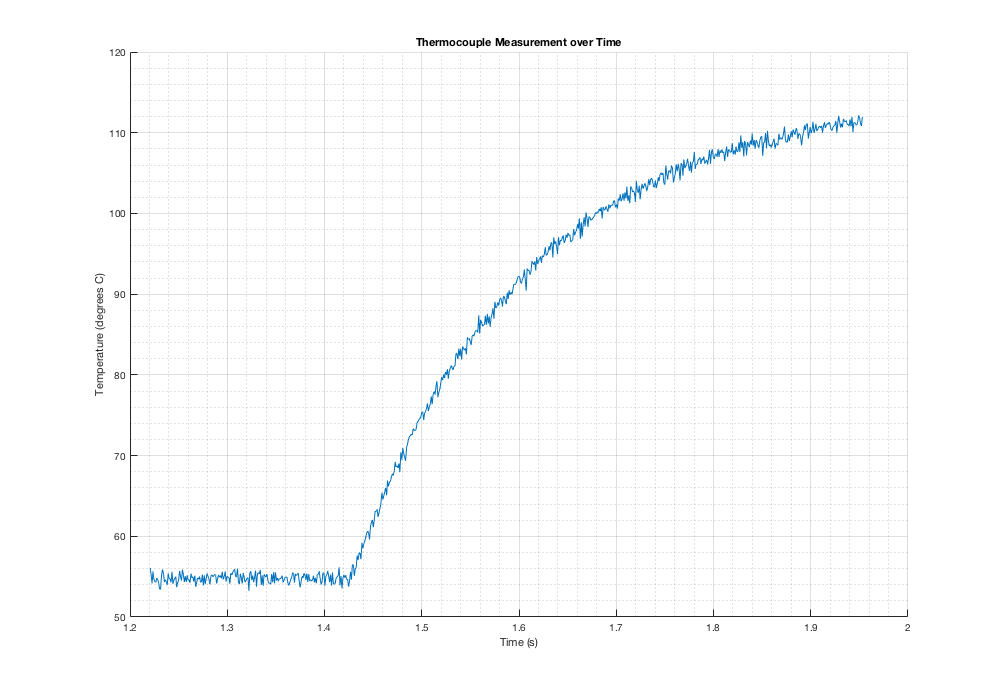
\includegraphics[height=2.0in]{/Users/noahstockwell/Documents/TeX/Proj544/Images/NoisyThermocouple.png}
	\caption{The signal over multiple samples}
\end{subfigure}%
~ 
\begin{subfigure}[t]{0.5\textwidth}
	\centering
	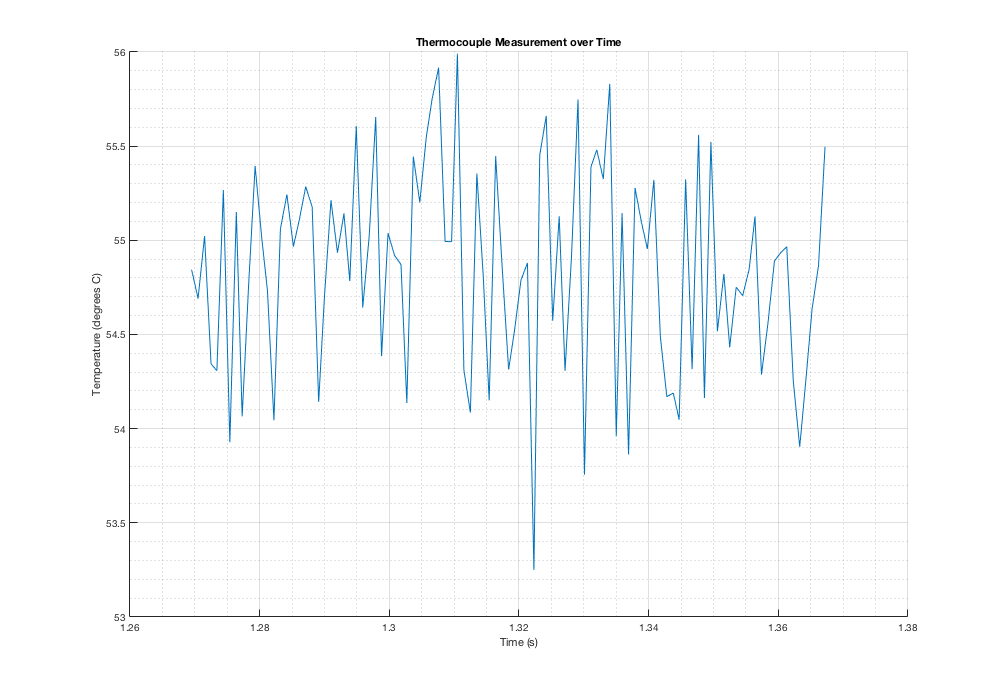
\includegraphics[height=2.0in]{/Users/noahstockwell/Documents/TeX/Proj544/Images/SmoothThermocouple.png}
	\caption{The signal over few samples}
\end{subfigure}
\caption{A sample thermocouple response at different sampling levels}
\end{figure}

Above in Figure 1(A), it is clear to us as humans the general shape of the generating signal. However, the true data points being collected look more like Figure 2(B) and it is often a trade-off between maintaining a close relationship to the original generating signal's value and maintaining a close relationship to the original generating signal's behavior. For example, as seen in section (2), the convolution with $\delta_n$ will either produce a function that has very few quick changes in its derivative, or a function that approximates the original function closely by value. It is in the Engineer's interest to ask the question: \textit{how much data can I reasonably destroy without jeopardizing the conclusion?}\\

With this in mind, we will construct a method and identify how `bad' it can be: how far can it be away from the generating signal?

\section{Formulation for $S\in C_0(\mathbb{R})$ using the Lebesgue Integral}
\subsection{Construction of problem}
Let $S$ be our observed signal. We can visualize $S$ as $S(t) = f(t) + \eta(t) + \rho(t)$ where $f$ is the exact representation of the real process, $\eta$ is white noise upon the signal, and $\rho$ is extreme instantaneous variation induced by the signal. To replicate the real world, let $\rho$ vanish everywhere except on a set of Lebesgue measure 0. The motivation for this representation is that it is possible to have extreme variation when recording a signal that has no physical meaning and does not repeat. As white noise on a signal is zero in the time domain, for all $E$ of sufficient measure, we would like $\displaystyle\int_E\eta=0$. We only need to consider $S$ supported on a set of finite measure as the time values sampled are discrete and thus extrapolation beyond local areas is not desired. As such, we only require $S$ to belong to $L^1_{\text{loc}}$.
\subsection{Requirements}
Without loss of generality, we can split $\eta$ into $\eta^+$ and $\eta^-$ such that:
\begin{align*}
\int S&=\int f+\int \eta\\\\
\int S&=\int f+\int \eta^+-\int \eta^-
\end{align*}
Where $\eta^+$ and $\eta^-$ are both strictly nonnegative functions on the signal interval I, and since we know $\eta$ should be zero in the time domain \cite{saito_naoki_simultaneous_1994}, we want to create a process such that:$$\int_I\eta^+=\int_I\eta^-$$
Since the $\eta^\pm$ are zero when the other is positive, we can let $$I=E^+\bigcup E^-$$ with $E^+$ and $E^-$ disjoint and thus we have:
$$\int_I\eta^i =\int_I\chi_{E^i}\cdot\eta^i= \int_{E^i}\eta^i$$
Since $E^i\subset I$. We can begin constructing the function by defining:
\begin{align*}
E_a^+ &= \{x: S(x)-f(x)>a\}\\
E_a^- &= \{x: f(x)-S(x)>a\}
\end{align*}
\vfill
Clearly, $E_a^+\nearrow E^+$ and $E_a^- \nearrow E^-$ as $a\to 0$. For almost everywhere compactly supported functions, we have $$m(E^\pm_a)\le m(E^\pm)\quad \forall\,\, a>0$$Similarly, for finitely supported functions, we have $$|E^\pm_a|\le |E^\pm|\quad \forall\,\, a>0$$
\vfill
With these, we want to optimize $f$ such that:
\begin{enumerate}
	\item The quantity of noise is largely time independent: 
	$$\lim_{a\to 0} \left\lvert m(E_a^+) - m(E_a^-) \right\rvert < \epsilon_a$$
	\item The amount of noise is largely time independent:
	$$\lim_{a\to 0}\left\lvert \int_{E_a^+} \eta - \int_{E_a^-} \eta\right\rvert<\epsilon_a$$
\end{enumerate}
We can rewrite (2) as:
$$\lim_{a\to 0}\left\lvert \int_{E_a^+} S(x)-f(x)\,dx - \int_{E_a^-} f(x)-S(x)\,dx\right\rvert<\epsilon_a$$
With these in hand, we now want to see how we can bound this difference. It is clear that we desire some type of average over value and time so that we can balance both requirement (1) and (2). This paper makes the choice to consider a convolution $\phi$ that is normalized and can be considered part of a sequence approaching an approximation to the identity. In fact, we will chose the exact $\phi_n$ that was selected earlier:

\begin{align*}
	\delta_n(x, w)&:=
	\begin{cases}
	\left(1-\left(\frac{x}{w}\right)^n\right)^2 & x\in (-w, w)\\
	0&x\not\in (-w, w)\\
	\end{cases}\\\\
	N(w)&:=\int_{-w}^w\delta_n(t, w)\,dt = C(w)\\\\
	\phi(x,w)&:= \frac{\delta_n(x,w)}{N(w)}
\end{align*}

The question is how far away from $f$ is $S \circledast \phi$? Two bounding options are considered.

\subsection{Error Bounding using a Naive Approach}
Because we require our convolution kernels to be normalized, we have:
\begin{align*}
	(S\circledast \phi_n) &= \int_E S(\tau)*\phi(x-\tau, w)\,d\tau\\
	 &\le \sup_{x\in E} S(x)\quad\\
\end{align*}
However, this bound is really not helpful. A smarter approach to bounding should be considered. One possible method would be to restrict ourselves to $A \subset E$:
\begin{align*}
(S\circledast \phi_n) &= \int_A S(\tau)*\phi(x-\tau, w)\,d\tau\\
&\le \sup_{x\in A_w} S(x)\quad\\
\end{align*}
Where $A_w$ is a $w$-dilation of $A$. This is a little more helpful but again $A$ has to be large enough to absorb $\eta$.

\subsection{Error Bounding using the Maximal Function}
The Hardy-Littlewood maximal function $S^*$ is defined to be:
\[
S^*(t) := \sup_{B_r(t)\,\, \forall t\in \mathbb{R}} \,\,\intbar_B S(t)\,dt 
\]
It is possible to put a bound on the maximal function, especially because we only consider a single-dimensional independent variable on $E$ with m$(E) < \infty$ \cite{stein_real_2006}:
\[
\text{m}({x\in E: S^*(x) > \alpha}) \le \frac{3}{\alpha} \norm{S}_{L^1(E)}
\]
It is apparent that we can consider the maximal function as the upper bound for the convolution if we require that the convolution kernel has most density around the origin and is only a small value away from vanishing outside of a small ball centered at the origin. In fact, with our choice of $\phi_n$ have:
\[
(S \circledast \phi_n)(t) \le (1+c) \,S^*(t)
\]
With $c>0$ small. In fact, because our convolution vanishes outside of a ball of radius $w$ around the origin and our convolution kernel is less than the box kernel $K$ of width $\le w$ outside of a smaller ball, we have:
\begin{align*}
(S\circledast \phi_n) &= \int_E S(\tau)*\phi(x-\tau, w)\,d\tau\\
& \le (1+c) \sup_{\tilde{w} \in (0,w]} \int_E S(\tau)*K(x-\tau, \tilde{w})\,d\tau\\
&=  (1+c) \sup_{B_r(t)\,\, \forall t\in (0, w]} \,\,\intbar_B S(t)\,dt\\
&= (1+c)\,S^*_{w}(x)
\end{align*}
Where $S^*_{w}(x)$ is the maximal function taken over balls of size up to $w$ around $x$ and $c>0$ small. This provides us a much nicer bound on the convolution.\\
It was claimed earlier that $S$ could be represented as the sum of three functions and $\rho$ vanishes everywhere except a set of Lebesgue measure 0. There are multiple methods to remove outliers for data: apply one or multiple and now we have:
\[
\int_E S = \int_E f + \eta
\]
as the Lebesgue integral ignores values on a set of measure zero. We can now assume that we can simply sum the convolution as we did in the beginning:
\begin{align*}
S(x)\approx(S\circledast\phi)(x, w) &\le \epsilon_0(x) + \sum_{a_n\in T_x} S\left(a_n\right)\int_{a_n}^{a_{n+1}} \phi(x-\tau, w)\,d\tau\\
&= \epsilon_0(x) + \sum_{a_n\in T_x} \left(f\left(a_n\right) + \eta\left(a_n\right)\right)\int_{a_n}^{a_{n+1}} \phi(x-\tau, w)\,d\tau\\
\end{align*}
If we set 
\[
b_{{a_n}(x), w} = \int_{a_n}^{a_{n+1}} \phi(x-\tau, w)\,d\tau
\]
we have
\begin{align*}
(S\circledast\phi)(x, w) &\le \epsilon_0(x) +  \sum_{a_n\in T_x} \left(f\left(a_n\right) + \eta\left(a_n\right)\right)\ * b_{{a_n}, w}(x)\\
&= \epsilon_0(x) +  \left(\sum_{a_n\in T_x} f\left(a_n\right) * b_{{a_n}, w}(x)\right) + \left(\sum_{a_n\in T_x} \eta\left(a_n\right) * b_{{a_n}, w}(x)\right)\\
\end{align*}
Since $\eta$ sums to zero in the time domain, we get:
\[
\sum_{a_n\in T_x} \eta\left(a_n\right) * b_{{a_n}, w}(x) \equiv 0
\]
Leaving us with only
\[
(S\circledast\phi)(x, w) \le \epsilon_0(x) +  \sum_{a_n\in T_x} f\left(a_n\right) * b_{{a_n}, w}(x)
\]
Which leads us back to the Riemann conclusion. At this point, the question is can we recover $f(t)$ exactly? Clearly we want equality, so the process would have to start with identifying $\epsilon_0$:
\[
\epsilon_0(x) = \min\left(\left|(1+c)*S^*_{w}(x) - S(x)\right|, \left|\sup_{\tilde{x}\in B_w(x)}S(\tilde{x}) - S(x)\right|\right)
\]
It should be clear at least with this choice of bounding, $f(t)$ cannot be recovered exactly.
\newpage
\section{Conclusion}
We do not have the ability to recreate $f$ with this formulation, however we may be able to get close for certain functions, especially simple functions. This process was implemented in MATLAB(\texttrademark) on an experiment involving temperature measurements of a thermocouple being moved from one environment to another:
\begin{figure}[H]
	\centering
	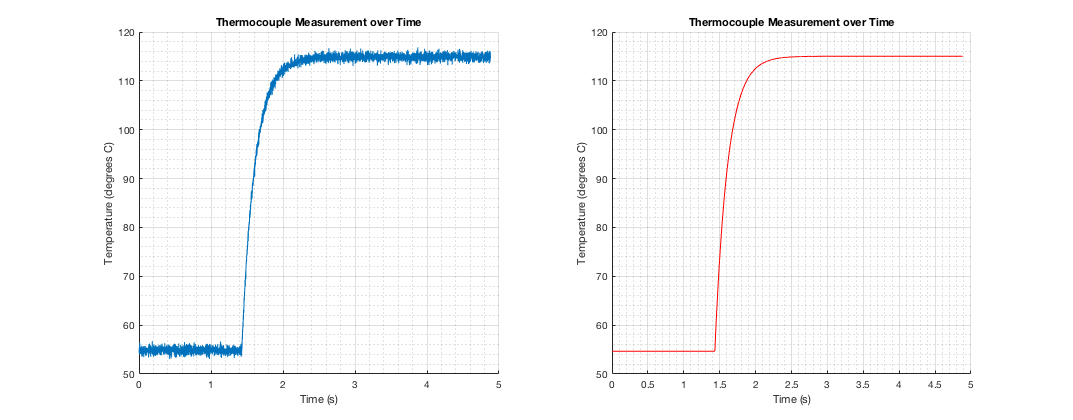
\includegraphics[height=2.0in]{/Users/noahstockwell/Documents/TeX/Proj544/Images/Comparison.png}
	\caption{Thermocouple response: Noisy and Convolved}
\end{figure}
Figure 2 demonstrates the potential of a well-tuned convolution in denoising signals for Engineering analysis. More work should be done to better identify the constant $c$ and if superior bounding methods exist.
\newpage
\bibliography{bibFile}
\bibliographystyle{plain}
\end{document}






